\documentclass[preprint,12pt]{elsarticle}

\usepackage[T1]{fontenc}
\usepackage[utf8]{inputenc}
\usepackage[english]{babel}
\usepackage{amsmath,amssymb}
\usepackage{graphicx}
\usepackage{booktabs}
\usepackage{array}
\usepackage{multirow}
\usepackage{siunitx}
\usepackage{xcolor}
\usepackage{hyperref}

\sisetup{
    detect-weight=true,
    table-number-alignment=center
}

\journal{Computerized Medical Imaging and Graphics}

\begin{document}
\begin{frontmatter}

\title{Detection-Guided Adaptive 2D Synthesis for Patient-Level Lung Malignancy Assessment from CT Volumes}

\author[1]{Domenico Paolo\corref{cor1}}
\author[1]{Alessandro Bria}
\author[1]{Claudio Marrocco}
\author[1]{Ciro Russo}
\author[1]{Marco Cantone}

\affiliation[1]{
    organization={Department of Electrical and Information Engineering, University of Cassino and Southern Latium},
    country={Italy}
}

\cortext[cor1]{Corresponding author}

\begin{abstract}
Patient-level malignancy assessment from lung CT requires integrating sparse evidence from pulmonary nodules distributed across a three-dimensional examination. Full-volume 3D neural networks preserve volumetric context, but their computational and memory requirements constrain resolution, batch size, and practical deployment. Conversely, fixed 2D projections and slice-selection strategies are efficient but may miss or dilute lesion-level evidence. We propose a detection-guided adaptive synthesis framework that converts a CT volume into a compact patient-specific 2D representation. A 3D nodule detector first localizes candidate nodules; the highest-confidence detections are then used as semantic control points for a radial basis function (RBF) surface. Sampling the preprocessed CT volume along this smooth surface yields a synthetic 2D image in which spatially distributed nodular evidence is concentrated for patient-level classification by standard 2D backbones. On LUNA16, using CPMNetv2 detections with threshold $0.50$ and top-$4$ candidates, the proposed Adaptive RBF representation with EfficientNetV2-S achieved a pooled AUC of $0.8149$, MCC of $0.4780$, and F1 score of $0.6806$ over 796 labeled scans. It significantly outperformed MIP axial projection (AUC $0.6075$), MIP tri-view (AUC $0.6175$), central axial slice selection (AUC $0.6153$), detector-crop MIL attention (AUC $0.5410$), fixed/random control-point ablations, and a full-volume 3D ResNet18 baseline (AUC $0.5659$). Paired DeLong tests confirmed significant AUC improvements over all planned comparators after FDR correction. These results suggest that the gain is not due merely to dimensionality reduction or 2D pretraining, but to lesion-guided adaptive sampling of the volume.
\end{abstract}

\begin{keyword}
Lung CT \sep Patient-level malignancy \sep Detection-guided synthesis \sep Adaptive projection \sep Radial basis functions
\end{keyword}

\end{frontmatter}

\section{Introduction}

Low-dose computed tomography (CT) is central to lung cancer screening because randomized screening trials have shown a lung-cancer mortality reduction compared with radiography or no screening~\cite{nlst2011,nelson2020}. CT screening reveals small pulmonary nodules at high spatial resolution, but the same volumetric richness makes automated patient-level prediction difficult. A CT examination may contain hundreds of axial slices, and the relevant evidence can consist of one or more nodules whose size, appearance, and location vary substantially across patients~\cite{armato2011lidc,setio2017luna16}. A model must therefore integrate sparse and spatially distributed findings while avoiding excessive sensitivity to irrelevant anatomy.

Deep learning has addressed this problem primarily through two families of representations. Full-volume 3D models preserve anatomical context and can learn directly from the CT volume, as shown by nodule-analysis and lung-cancer risk models based on volumetric CNNs~\cite{zhu2018deeplung,ardila2019endtoend,mikhael2023sybil}. However, dense 3D processing remains expensive to train and deploy. Its memory footprint often forces compromises in spatial resolution, batch size, or model capacity. In contrast, 2D and multi-view methods use fixed projections, selected slices, or local nodule crops to exploit efficient image backbones~\cite{setio2016multiview,zheng2020mip,jang2022m3t}. These strategies are computationally attractive, but a fixed sampling geometry is not necessarily aligned with the lesion configuration of each patient. Small nodules may be missed, multiple lesions may be projected into ambiguous structures, and diagnostically important regions may occupy only a small fraction of the final image.

This work studies patient-level malignancy assessment as an adaptive representation problem. Rather than classifying the full 3D scan or applying the same 2D projection to every patient, we first localize nodules using a 3D detector and then synthesize a patient-specific 2D image from the volume. The detector follows the center-points matching family of anchor-free 3D nodule detectors~\cite{song2020cpm,luo2022scpmnet}. Its outputs define control points for a smooth radial basis function (RBF) surface, a classical tool for scattered-data interpolation~\cite{powell1987rbf}. The surface bends through the CT volume toward the most relevant candidates, and sampling along this surface creates a compact representation that concentrates nodular evidence while preserving enough spatial context for a 2D classifier.

The resulting pipeline separates volumetric localization from patient-level classification. The 3D detector is used once to identify candidate lesions and define the adaptive surface; thereafter, classification operates on a single 2D image. This design also addresses a natural alternative based on multiple-instance learning, where detected candidates are classified independently and pooled at patient level~\cite{ilse2018attention}. In contrast, the proposed representation preserves a direct visual link between detector outputs, control points, sampling surface, and final synthetic image, while remaining reusable across backbones and experimental settings.

The main contributions are:
\begin{itemize}
    \item We introduce a detection-guided adaptive 3D-to-2D synthesis framework for patient-level lung malignancy assessment.
    \item We formulate synthetic image generation as RBF surface interpolation from detector-derived control points, enabling patient-specific volumetric sampling.
    \item We evaluate the method against non-adaptive 2D baselines, detector-crop multiple-instance learning, fixed/random control-point ablations, Shepard interpolation, and a full-volume 3D ResNet18 baseline.
    \item We provide paired statistical testing and computational analysis, separating classifier-side cost from detector-inclusive cost.
\end{itemize}

\section{Related Work}

\subsection{Volumetric lung CT analysis}

Early deep learning systems for lung CT combined nodule detection with local or patient-level classification. DeepLung used 3D detection followed by 3D feature extraction for nodule diagnosis~\cite{zhu2018deeplung}. End-to-end systems have subsequently shown that volumetric CT can support lung cancer risk prediction from current and prior scans~\cite{ardila2019endtoend}, and Sybil demonstrated multi-year risk prediction from a single low-dose CT~\cite{mikhael2023sybil}. These methods show the value of volumetric context, but dense 3D processing remains computationally demanding, especially when high-resolution input volumes are required.

\subsection{2D projections and multi-view representations}

Efficient alternatives represent CT volumes through 2D observations. Multi-view CNNs have been used for nodule false-positive reduction~\cite{setio2016multiview}, and hybrid 2D/3D architectures aggregate information across planes or slices~\cite{jang2022m3t}. Maximum intensity projections (MIPs) are clinically meaningful in lung imaging because they can enhance high-attenuation nodules relative to lung parenchyma~\cite{zheng2020mip}. However, fixed axial, tri-view, or central-slice representations do not adapt to patient-specific lesion locations. Our approach retains the efficiency of 2D classification while making the sampling geometry dependent on detected nodules.

\subsection{Detection-guided patient-level reasoning}

Nodule detectors provide an explicit mechanism for focusing computation on sparse regions of interest. SCPM-Net represents nodules as bounding spheres and detects them through center-point matching~\cite{luo2022scpmnet}. CPMNetv2 further improves this family of detectors with practical training and inference refinements. A natural baseline is therefore to crop detected candidates and aggregate their predictions using mean, max, or attention pooling. In contrast, our method does not classify each candidate independently. It uses the detections to construct a shared patient-level surface, allowing the downstream classifier to observe multiple lesions and surrounding context in a single image.

\subsection{Adaptive geometric synthesis}

Radial basis functions are widely used to interpolate smooth functions from scattered control points. Given control points $\mathbf{p}_i=(x_i,y_i)$ and target depths $z_i$, the RBF surface can be written as
\begin{equation}
    S(x,y) = \sum_{i=1}^{N} w_i \, \phi\left(\left\|(x,y)-\mathbf{p}_i\right\|\right) + a_0 + a_1 x + a_2 y,
\end{equation}
where $\phi(\cdot)$ is the radial kernel and the affine term captures low-frequency variation. Here, the control points are derived from detector candidates and their local neighborhoods. The surface $S$ defines, for each image location $(x,y)$, the axial coordinate from which the CT intensity is sampled. Because the synthesized image is generated from a single-valued surface $z=S(x,y)$, two candidates with the same projected $(x,y)$ location but different axial coordinates cannot both be represented at that pixel. We therefore remove projected duplicates before surface fitting, retaining the highest-priority candidate, based on malignancy score when available and otherwise detector probability. This converts sparse 3D detections into a dense 2D representation while maintaining a smooth and interpretable sampling geometry.

As a second adaptive interpolation strategy, we also evaluated Shepard interpolation~\cite{shepard1968}. Shepard interpolation estimates the surface value as an inverse-distance weighted average of the control-point depths:
\begin{equation}
    S_{\mathrm{Shepard}}(x,y) =
    \frac{\sum_{i=1}^{N} d_i(x,y)^{-p} z_i}
         {\sum_{i=1}^{N} d_i(x,y)^{-p}},
    \quad
    d_i(x,y)=\left\|(x,y)-\mathbf{p}_i\right\|.
\end{equation}
Unlike the RBF formulation, which solves for a globally smooth surface with an affine component, Shepard interpolation is local and gives more influence to nearby control points. In this study, Shepard uses the same detector-selected candidates and working point as RBF; it is therefore an adaptive comparator that isolates the effect of the interpolation rule while keeping detector guidance fixed. For Shepard, each retained candidate is represented as a disk centered at $(x_i,y_i,z_i)$ with the predicted detector radius, and overlapping disks in the $(x,y)$ plane are removed before interpolation to avoid assigning conflicting depths to the same projected region.

\section{Materials and Methods}

\subsection{Dataset and labels}

Experiments were performed on LUNA16~\cite{setio2017luna16}, a curated subset of LIDC-IDRI~\cite{armato2011lidc}. LUNA16 contains 888 CT scans and 1,186 reference nodules with diameter at least 3 mm accepted by at least three of four radiologists. CT volumes were preprocessed to 1 mm isotropic spacing and lung-focused crops, matching the preprocessing used by the detector and synthetic image generation pipeline.

Because LUNA16 is primarily a detection benchmark, patient-level labels were derived from the corresponding LIDC-IDRI malignancy ratings. For each scan, available nodule malignancy scores were averaged. Scans with mean malignancy below 3 were labeled benign, scans above 3 were labeled malignant, and scans with mean malignancy equal to 3 were excluded as indeterminate. This produced 796 labeled scans, including 320 malignant and 476 benign cases.

\subsection{Detector and working point}

We used CPMNetv2 as the nodule detector and evaluated it in a 10-fold setting on LUNA16. The detector outputs candidate centers, radii, and probabilities in the preprocessed voxel space. The pooled test FROC obtained by concatenating predictions and ground truth over the 10 folds is reported in Table~\ref{tab:detector_froc}. The pooled mean FROC was $0.8017$.

\begin{table}[t]
\centering
\caption{Pooled CPMNetv2 FROC on LUNA16 over the 10 test folds.}
\label{tab:detector_froc}
\begin{tabular}{lrrrrrrr}
\toprule
FP/scan & 0.125 & 0.25 & 0.5 & 1 & 2 & 4 & 8 \\
\midrule
Sensitivity & 0.499 & 0.644 & 0.765 & 0.852 & 0.921 & 0.954 & 0.977 \\
\bottomrule
\end{tabular}
\end{table}

For synthesis, the detector operating point was selected under a representation-budget criterion rather than by maximizing detection sensitivity alone. This distinction is important because each retained detection becomes a geometric control region for the adaptive surface. False-positive detections are therefore not merely additional candidates: they can deform the sampling surface toward non-informative anatomy and dilute the lesion-aware representation. We consequently constrained the number of retained detections with a small top-$k$ budget and imposed a minimum confidence threshold.

Table~\ref{tab:coverage_budget} summarizes the coverage--false-positive trade-off for the selected threshold range. The final working point, probability threshold $0.50$ and top-$4$ detections per scan, covers 986 of 1,186 annotated nodules ($83.14\%$) and 586 of 601 positive scans ($97.50\%$), while keeping the false-positive burden close to the intended budget of 2 FP/scan. Increasing top-$k$ improves nodule coverage, but it also introduces additional false-positive control regions. The working point was fixed before training the downstream classifiers.

\begin{table}[t]
\centering
\caption{Detector coverage analysis used to select the synthesis working point. Coverage is computed after applying the probability threshold and retaining the top-$k$ detections per scan. A nodule is considered covered when one selected detection center falls inside its annotated radius.}
\label{tab:coverage_budget}
\resizebox{\linewidth}{!}{%
\begin{tabular}{rrrrrr}
\toprule
Threshold & Top-$k$ & Nodule coverage & Positive-scan coverage & FP/scan & Detections kept \\
\midrule
0.50 & 2 & 66.44 & 95.84 & 0.93 & 1,615 \\
0.50 & 3 & 76.73 & 97.17 & 1.52 & 2,274 \\
\textbf{0.50} & \textbf{4} & \textbf{83.14} & \textbf{97.50} & \textbf{2.05} & \textbf{2,804} \\
0.50 & 5 & 86.85 & 98.00 & 2.48 & 3,236 \\
0.50 & 6 & 89.46 & 98.00 & 2.85 & 3,590 \\
0.45 & 4 & 83.31 & 97.84 & 2.29 & 3,020 \\
0.40 & 4 & 83.39 & 97.84 & 2.54 & 3,243 \\
\bottomrule
\end{tabular}
}
\end{table}

\subsection{Adaptive RBF synthesis}

For each scan, the detector candidates surviving the selected working point define the primary control regions. For RBF, every retained detection contributes five control points: the detected center plus four contour points placed on the predicted-radius circle in the axial plane at angles $0$, $\pi/2$, $\pi$, and $3\pi/2$. These contour points constrain the fitted surface around the local spatial extent of the candidate rather than only at its center. All control points are clipped to the preprocessed volume bounds. For Shepard, the same retained detections are represented as radius-aware disks, so the interpolation uses the candidate extent directly through the disk radius. The resulting surface is estimated over the axial image plane and returns a depth value for each pixel. The preprocessed CT volume is then sampled at these depths to generate a single synthetic 2D image. Unless otherwise stated, synthetic images were resized to $256 \times 384$ and represented as three-channel images for compatibility with ImageNet-pretrained backbones.

Figure~\ref{fig:method} illustrates the proposed pipeline: the preprocessed CT volume is processed by a detector, detections are converted into control points, an adaptive RBF surface is fitted, and the final synthetic 2D image is classified at the patient level.

\begin{figure}[t]
    \centering
    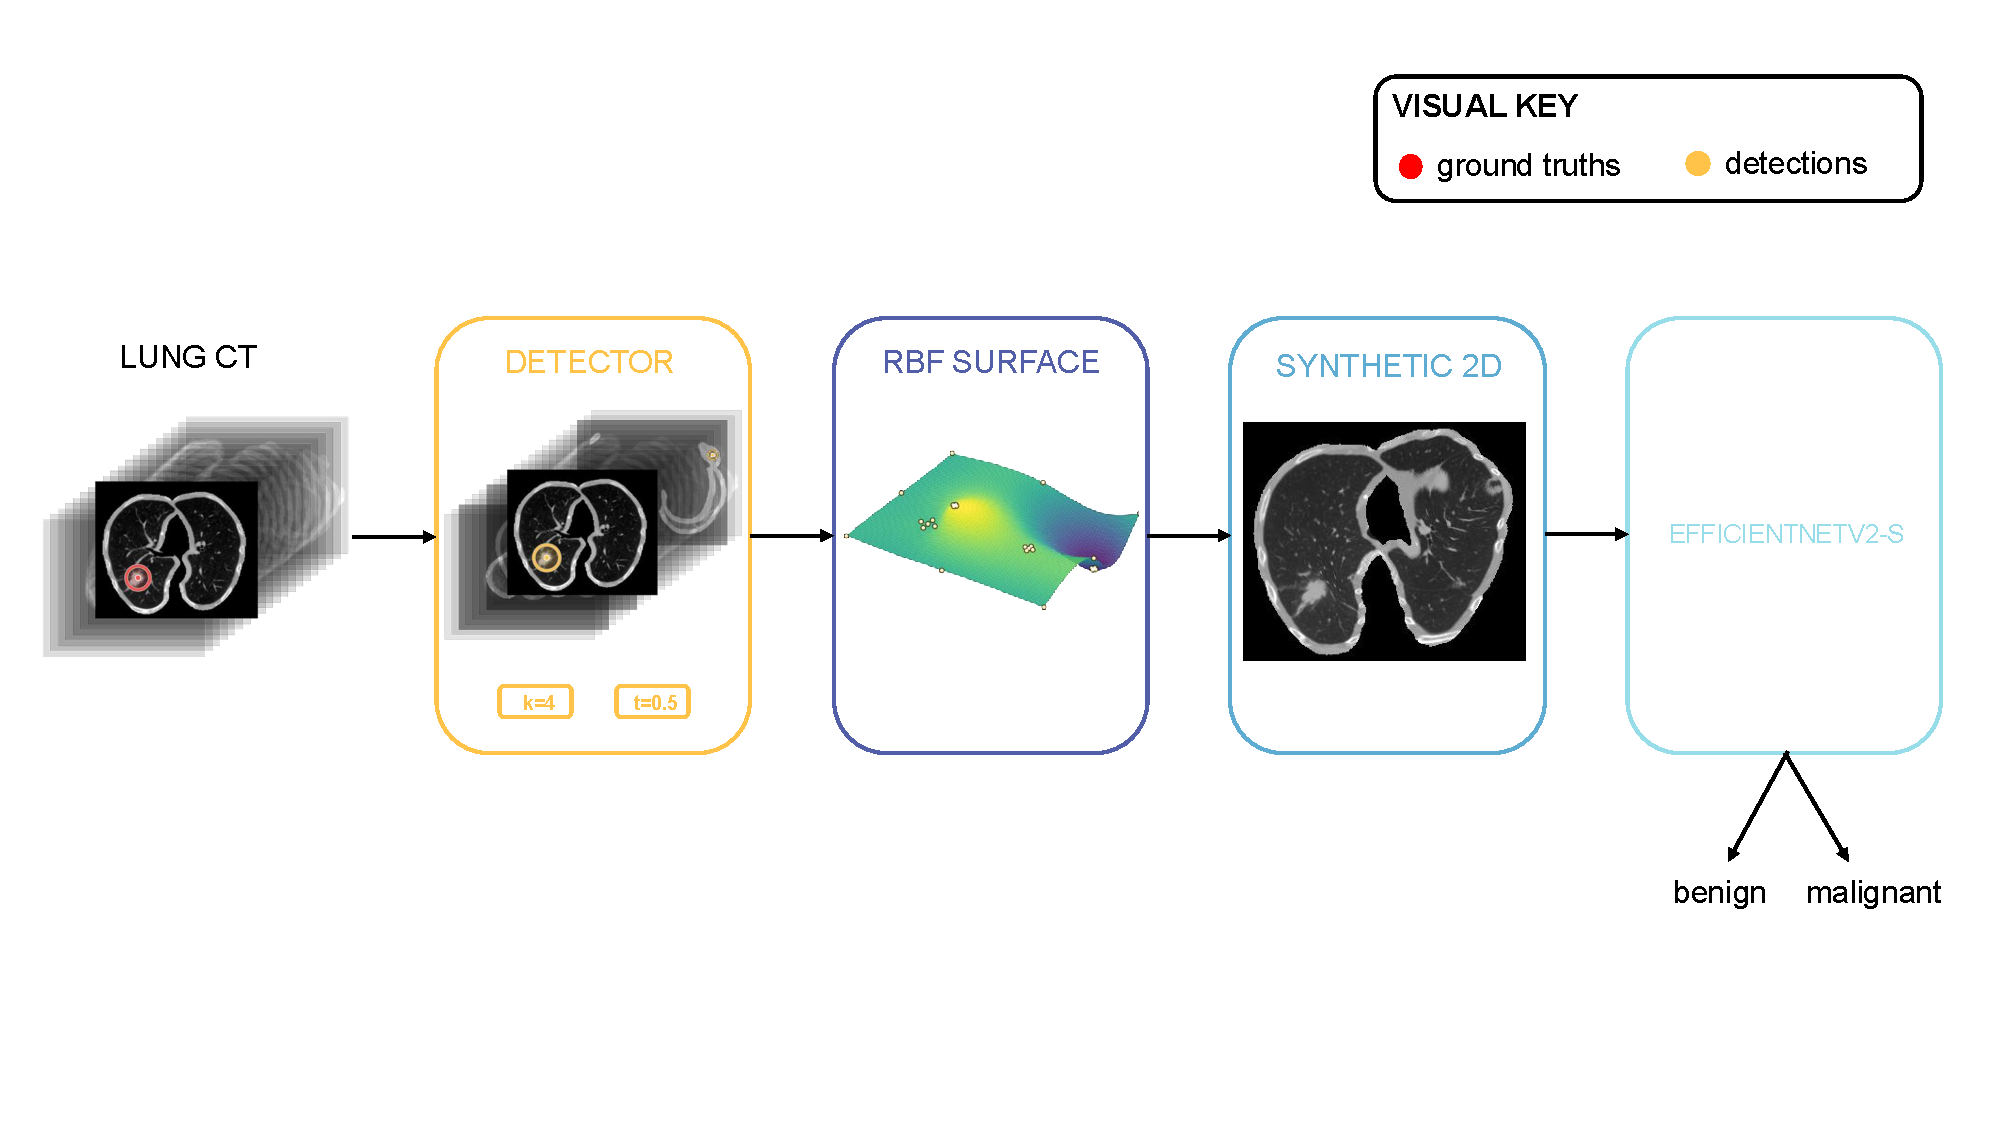
\includegraphics[width=\linewidth]{figures/Method.pdf}
    \caption{Overview of the proposed detection-guided adaptive synthesis framework. CPMNetv2 identifies candidate nodules in the preprocessed CT volume. The selected detections define control points for an RBF surface, which samples the volume to produce a compact synthetic 2D representation for patient-level malignancy classification.}
    \label{fig:method}
\end{figure}

\subsection{Baselines and ablations}

We compared the proposed representation against several baselines designed to isolate the role of detector-guided geometry:
\begin{itemize}
    \item \textbf{MIP axial and MIP tri-view:} fixed non-adaptive maximum intensity projection baselines.
    \item \textbf{Central axial slice:} a single fixed anatomical slice from the preprocessed volume.
    \item \textbf{Detector crop-MIL:} top-$4$ detector-centered 2D crops processed by the same encoder and aggregated with attention.
    \item \textbf{Fixed-control and random-control RBF:} RBF surfaces generated without detector-guided control-point placement.
    \item \textbf{Adaptive Shepard:} the same detector-guided working point using Shepard interpolation instead of RBF.
    \item \textbf{3D ResNet18:} a full-volume baseline trained on fit-padded $224 \times 288 \times 288$ inputs.
\end{itemize}

All main 2D classifiers used EfficientNetV2-S unless otherwise specified. Results are reported as pooled metrics by concatenating predictions from the 10 test folds. AUC was computed from pooled continuous scores, while MCC, accuracy, F1, precision, and recall were computed from pooled binary predictions.

\subsection{Statistical analysis}

The unit of analysis was the scan-level prediction. We compared the proposed Adaptive RBF model against planned comparators using paired DeLong tests for AUC and exact McNemar/binomial tests for binary prediction disagreement. Confidence intervals were estimated using stratified patient-level bootstrap with 5,000 resamples. Multiple comparisons were corrected using Benjamini--Hochberg false discovery rate (FDR).

\section{Results}

\subsection{Patient-level classification}

Table~\ref{tab:main_results} reports pooled patient-level classification performance. The proposed Adaptive RBF representation with EfficientNetV2-S achieved the best AUC ($0.8149$), MCC ($0.4780$), and F1 score ($0.6806$). Non-adaptive 2D projections remained near AUC $0.61$, while fixed and random control-point RBF ablations performed similarly to these baselines. The detector-crop MIL attention baseline did not close the gap, suggesting that simply classifying detected candidates independently is not sufficient for this patient-level task.

\begin{table}[t]
\centering
\caption{Pooled patient-level classification results over the 10 LUNA16 test folds. All methods use EfficientNetV2-S unless otherwise noted.}
\label{tab:main_results}
\resizebox{\linewidth}{!}{%
\begin{tabular}{llrrrr}
\toprule
Family & Method & AUC & MCC & F1 & Accuracy \\
\midrule
Proposed & Adaptive RBF & \textbf{0.8149} & \textbf{0.4780} & \textbf{0.6806} & 0.7513 \\
Adaptive & Adaptive Shepard & 0.7793 & 0.4308 & 0.6283 & 0.7324 \\
Non-adaptive & MIP tri-view & 0.6175 & 0.1556 & 0.5008 & 0.5917 \\
Non-adaptive & Central axial slice & 0.6153 & 0.1610 & 0.4668 & 0.6068 \\
Non-adaptive & MIP axial & 0.6075 & 0.1604 & 0.5061 & 0.5930 \\
Ablation & Random-control RBF & 0.6105 & 0.1877 & 0.5207 & 0.6068 \\
Ablation & Fixed-control RBF & 0.5878 & 0.1109 & 0.4499 & 0.5791 \\
MIL baseline & Detector crop-MIL attention & 0.5410 & 0.1861 & 0.5942 & 0.4510 \\
3D baseline & ResNet18 fit-pad & 0.5659 & 0.0989 & 0.4870 & 0.5553 \\
\bottomrule
\end{tabular}
}
\end{table}

The strongest detector-guided synthetic configuration was RBF with EfficientNetV2-S. Table~\ref{tab:backbones} shows that RBF remained competitive across multiple 2D backbones, while Shepard interpolation was generally lower in AUC. DenseNet121 with RBF achieved AUC $0.7989$, and VGG16 with RBF achieved AUC $0.7754$.

\begin{table}[t]
\centering
\caption{Backbone comparison for detector-guided synthetic images generated with threshold $0.50$ and top-$4$ detections.}
\label{tab:backbones}
\resizebox{0.92\linewidth}{!}{%
\begin{tabular}{llrrrr}
\toprule
Interpolation & Backbone & AUC & MCC & F1 & Recall \\
\midrule
RBF & EfficientNetV2-S & \textbf{0.8149} & \textbf{0.4780} & \textbf{0.6806} & \textbf{0.6594} \\
RBF & DenseNet121 & 0.7989 & 0.4487 & 0.6624 & 0.6406 \\
Shepard & EfficientNetV2-S & 0.7793 & 0.4308 & 0.6283 & 0.5625 \\
Shepard & ResNet50 & 0.7784 & 0.4256 & 0.6376 & 0.5938 \\
RBF & VGG16 & 0.7754 & 0.4568 & 0.6677 & 0.6469 \\
RBF & EfficientNet-B0 & 0.7701 & 0.4155 & 0.6442 & 0.6281 \\
RBF & ResNet50 & 0.7658 & 0.4122 & 0.6361 & 0.6062 \\
RBF & ResNet18 & 0.7622 & 0.4050 & 0.6378 & 0.6219 \\
\bottomrule
\end{tabular}
}
\end{table}

\subsection{Statistical comparisons}

Table~\ref{tab:stats} summarizes paired comparisons versus Adaptive RBF. The proposed method significantly improved AUC over all planned comparators after FDR correction. The comparison with Shepard interpolation was significant for AUC ($p=0.0255$), although McNemar's test was not significant, indicating that RBF primarily improved ranking/discrimination rather than producing a clearly different binary error set at the selected decision threshold.

\begin{table}[t]
\centering
\caption{Paired statistical comparisons against Adaptive RBF. Positive $\Delta$ indicates improvement of Adaptive RBF over the comparator.}
\label{tab:stats}
\resizebox{\linewidth}{!}{%
\begin{tabular}{lrrrr}
\toprule
Comparator & $\Delta$ AUC & DeLong $p$ & FDR $p$ & $\Delta$ MCC \\
\midrule
Adaptive Shepard & 0.0356 & $2.55{\times}10^{-2}$ & $2.55{\times}10^{-2}$ & 0.0471 \\
MIP axial & 0.2074 & $2.05{\times}10^{-19}$ & $4.10{\times}10^{-19}$ & 0.3175 \\
MIP tri-view & 0.1974 & $9.09{\times}10^{-17}$ & $1.45{\times}10^{-16}$ & 0.3223 \\
Central axial slice & 0.1996 & $1.12{\times}10^{-16}$ & $1.50{\times}10^{-16}$ & 0.3170 \\
Detector crop-MIL attention & 0.2740 & $2.87{\times}10^{-62}$ & $2.30{\times}10^{-61}$ & 0.2919 \\
Fixed-control RBF & 0.2271 & $1.24{\times}10^{-20}$ & $3.31{\times}10^{-20}$ & 0.3670 \\
Random-control RBF & 0.2045 & $1.72{\times}10^{-16}$ & $1.96{\times}10^{-16}$ & 0.2903 \\
3D ResNet18 fit-pad & 0.2491 & $1.06{\times}10^{-23}$ & $4.23{\times}10^{-23}$ & 0.3790 \\
\bottomrule
\end{tabular}
}
\end{table}

\subsection{Computational profile}

The proposed representation compresses each preprocessed CT scan into a single $3 \times 256 \times 384$ image. The 3D ResNet18 baseline uses a $1 \times 224 \times 288 \times 288$ volume, corresponding to approximately $63\times$ more scalar input values before accounting for intermediate 3D activations. At the classifier stage, EfficientNetV2-S requires 11.15 GFLOPs for the adaptive 2D image, whereas the 3D ResNet18 forward pass requires 7359.84 GFLOPs. Detector-crop MIL requires up to four 2D encoder passes per patient.

When detector inference is included, the adaptive pipeline is dominated by CPMNetv2 sliding-window inference. CPMNetv2 uses $64 \times 128 \times 128$ crops with stride $48 \times 96 \times 96$, resulting in a mean of 48.40 crops per scan. This corresponds to an average detector-inclusive cost of 33282.75 GFLOPs per scan. This cost should be interpreted as a reusable preprocessing step: the same detections support FROC evaluation, working-point selection, coverage analysis, synthetic generation, and detector-crop baselines.

\section{Discussion}

The results support the central hypothesis that effective 3D-to-2D compression for patient-level malignancy assessment should be lesion-aware. Fixed MIP and central-slice baselines reduce the computational burden, but their sampling geometry is independent of the patient's nodules and therefore dilutes the relevant signal. Fixed-control and random-control RBF ablations further show that the benefit is not explained merely by applying a smooth surface or by using a pretrained 2D backbone. Performance improves only when the surface is guided by detector-derived control points.

The detector-crop MIL baseline addresses an important alternative interpretation: if the detector already localizes nodules, perhaps classifying each candidate independently and aggregating predictions is sufficient. Its lower AUC suggests that the adaptive surface provides useful patient-level context beyond isolated crops. The synthetic image can expose several detected regions and their surrounding anatomy to a single classifier, while still avoiding full-volume inference.

RBF outperformed Shepard interpolation in AUC. This suggests that the smoother global behavior of the RBF surface may provide a more stable representation for downstream ranking, although the non-significant McNemar test between RBF and Shepard indicates that their thresholded decisions remain relatively close. From a methodological perspective, Shepard interpolation remains a useful ablation, but RBF is the more appropriate default for the proposed representation.

The computational analysis reveals a nuanced trade-off. If synthetic images and detections are precomputed, the classifier-side cost is comparable to ordinary 2D baselines and far below full-volume 3D classification. If processing begins from raw/preprocessed CT volumes, detector inference dominates the adaptive pipeline. This is not a weakness to hide: the method intentionally uses 3D computation for the task where it is most valuable, localization, and then reuses that intermediate representation for efficient patient-level learning.

\section{Limitations}

This study has several limitations. First, patient-level labels are derived from LIDC-IDRI nodule malignancy ratings rather than from longitudinal clinical outcomes or histopathology, and indeterminate cases were excluded. Second, all experiments were performed on LUNA16/LIDC-derived data; external validation is necessary before clinical claims can be made. Third, the adaptive representation depends on detector quality. Missed nodules or poorly localized candidates can affect the synthesized image. Fourth, although classifier-side inference is efficient, detector-inclusive inference remains computationally expensive because of sliding-window 3D detection. Finally, the current framework synthesizes a single 2D image per scan; future work could study uncertainty-aware multi-surface synthesis or joint optimization of detector and classifier.

\section{Conclusion}

We presented a detection-guided adaptive RBF synthesis framework for patient-level lung malignancy assessment from CT volumes. By converting detector outputs into a smooth patient-specific sampling surface, the method concentrates volumetric nodular evidence into a compact 2D image suitable for efficient classification. On LUNA16, Adaptive RBF with EfficientNetV2-S achieved AUC $0.8149$ and significantly outperformed non-adaptive 2D projections, detector-crop MIL, unguided RBF ablations, Shepard interpolation, and a full-volume 3D ResNet18 baseline. These findings indicate that the key advantage lies not in reducing 3D CT to 2D per se, but in using detector-guided geometry to decide how the reduction is performed.

\begin{thebibliography}{99}
\bibitem{nlst2011}
National Lung Screening Trial Research Team,
\newblock Reduced lung-cancer mortality with low-dose computed tomographic screening,
\newblock \emph{New England Journal of Medicine}, 365(5):395--409, 2011.

\bibitem{nelson2020}
H.~J. de Koning et al.,
\newblock Reduced lung-cancer mortality with volume CT screening in a randomized trial,
\newblock \emph{New England Journal of Medicine}, 382(6):503--513, 2020.

\bibitem{armato2011lidc}
S.~G. Armato III et al.,
\newblock The Lung Image Database Consortium (LIDC) and Image Database Resource Initiative (IDRI): A completed reference database of lung nodules on CT scans,
\newblock \emph{Medical Physics}, 38(2):915--931, 2011.

\bibitem{setio2017luna16}
A.~A.~A. Setio et al.,
\newblock Validation, comparison, and combination of algorithms for automatic detection of pulmonary nodules in computed tomography images: The LUNA16 challenge,
\newblock \emph{Medical Image Analysis}, 42:1--13, 2017.

\bibitem{zhu2018deeplung}
W.~Zhu, C.~Liu, W.~Fan, and X.~Xie,
\newblock DeepLung: Deep 3D dual path nets for automated pulmonary nodule detection and classification,
\newblock in \emph{Proc. IEEE Winter Conference on Applications of Computer Vision}, pp.~673--681, 2018.

\bibitem{ardila2019endtoend}
D.~Ardila et al.,
\newblock End-to-end lung cancer screening with three-dimensional deep learning on low-dose chest computed tomography,
\newblock \emph{Nature Medicine}, 25:954--961, 2019.

\bibitem{mikhael2023sybil}
P.~G. Mikhael et al.,
\newblock Sybil: A validated deep learning model to predict future lung cancer risk from a single low-dose chest computed tomography,
\newblock \emph{Journal of Clinical Oncology}, 41(12):2191--2200, 2023.

\bibitem{song2020cpm}
T.~Song et al.,
\newblock CPM-Net: A 3D center-points matching network for pulmonary nodule detection in CT scans,
\newblock in \emph{Medical Image Computing and Computer Assisted Intervention -- MICCAI 2020}, pp.~550--559, 2020.

\bibitem{setio2016multiview}
A.~A.~A. Setio et al.,
\newblock Pulmonary nodule detection in CT images: False positive reduction using multi-view convolutional networks,
\newblock \emph{IEEE Transactions on Medical Imaging}, 35(5):1160--1169, 2016.

\bibitem{zheng2020mip}
S.~Zheng, X.~Cui, M.~Vonder, R.~N.~J. Veldhuis, Z.~Ye, R.~Vliegenthart, M.~Oudkerk, and P.~M.~A. van Ooijen,
\newblock Deep learning-based pulmonary nodule detection: Effect of slab thickness in maximum intensity projections at the nodule candidate detection stage,
\newblock \emph{Computer Methods and Programs in Biomedicine}, 196:105620, 2020.

\bibitem{jang2022m3t}
J.~Jang and D.~Hwang,
\newblock M3T: Three-dimensional medical image classifier using multi-plane and multi-slice transformer,
\newblock in \emph{Proc. IEEE/CVF Conference on Computer Vision and Pattern Recognition}, pp.~20686--20697, 2022.

\bibitem{luo2022scpmnet}
X.~Luo, T.~Song, G.~Wang, J.~Chen, Y.~Chen, K.~Li, D.~N. Metaxas, and S.~Zhang,
\newblock SCPM-Net: An anchor-free 3D lung nodule detection network using sphere representation and center points matching,
\newblock \emph{Medical Image Analysis}, 75:102287, 2022.

\bibitem{powell1987rbf}
M.~J.~D. Powell,
\newblock Radial basis functions for multivariable interpolation: A review,
\newblock in \emph{Algorithms for Approximation}, pp.~143--167, Clarendon Press, 1987.

\bibitem{shepard1968}
D.~Shepard,
\newblock A two-dimensional interpolation function for irregularly-spaced data,
\newblock in \emph{Proceedings of the 1968 23rd ACM National Conference}, pp.~517--524, 1968.

\bibitem{ilse2018attention}
M.~Ilse, J.~M. Tomczak, and M.~Welling,
\newblock Attention-based deep multiple instance learning,
\newblock in \emph{Proceedings of the 35th International Conference on Machine Learning}, PMLR 80:2127--2136, 2018.
\end{thebibliography}

\end{document}
